%% why_comparative_genomics.tex
%% Copyright: James Hutton Institute 2016
%% Author: Leighton Pritchard
%% Why Comparative Genomics?

% WHY COMPARATIVE GENOMICS
\begin{frame}
  \frametitle{Why comparative genomics?}
    \begin{columns}[c] 
      \column{.6\textwidth} 
        \begin{itemize}
         \item \textcolor{hutton_green}{Transfer functional information from model systems (\textit{E. coli}, \textit{A. thaliana}, \textit{D. melanogaster}) to non-model systems}        
         \item \textcolor{hutton_blue}{Genome similarity $\propto$ phenotype? (\textit{functional genomics}): virulence and host range}         
         \item \textcolor{RawSienna}{Genome similarity $\propto$ relatedness? (\textit{phylogenomics}): record of evolutionary processes and constraints}
        \end{itemize}
      \column{.4\textwidth}
        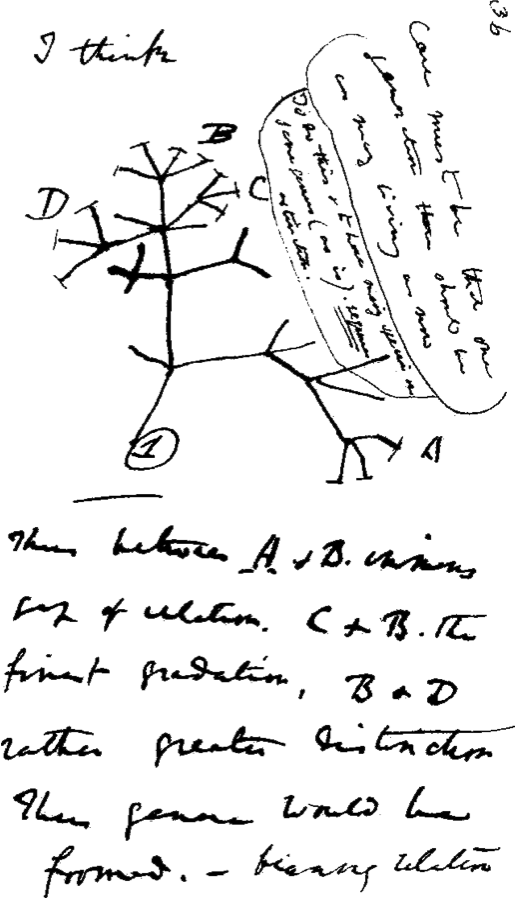
\includegraphics[width=\textwidth]{images/darwin_tree}
    \end{columns}  
\end{frame}

% WHY COMPARATIVE GENOMICS
\begin{frame}
  \frametitle{Genomes aren't everything$\ldots$}
    \begin{columns}[c] 
      \column{.6\textwidth} 
        \begin{alertblock}{Context}
          \begin{itemize}
            \item epigenetics
            \item tissue differentiation/differential expression
            \item mesoscale systems, etc.
          \end{itemize}
        \end{alertblock}
        \begin{block}{Phenotypic plasticity, responses to}         
          \begin{itemize}
            \item temperature
            \item stress
            \item community, etc.
          \end{itemize}
        \end{block}
        \textcolor{red}{$\ldots$and therefore systems biology$\ldots$}
      \column{.4\textwidth}
        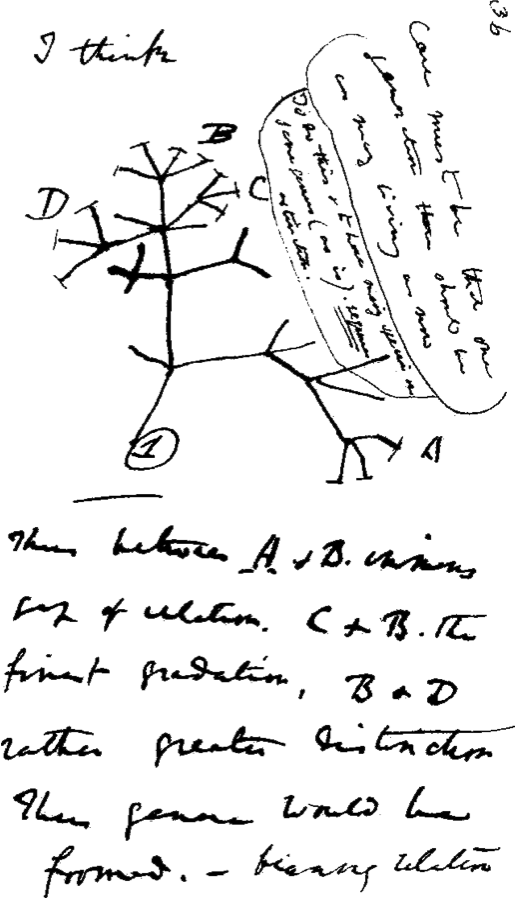
\includegraphics[width=\textwidth]{images/darwin_tree}
    \end{columns}  
\end{frame}

% LEVELS OF COMPARISON
\begin{frame}
  \frametitle{Levels of comparison}
    \begin{alertblock}{Bulk Properties}
      \begin{itemize}
        \item \textcolor{hutton_green}{e.g. $k$-mer spectra} (\textcolor{hutton_purple}{\href{https://github.com/marbl/Mash}{MaSH}}, \textcolor{hutton_purple}{\href{https://github.com/dkoslicki/MetaPalette}{MetaPalette}}, etc.)
      \end{itemize}
    \end{alertblock}
    \begin{block}{Whole Genome Sequence}
      \begin{itemize}
        \item \textcolor{hutton_blue}{sequence similarity} (\textcolor{hutton_purple}{\href{https://blast.ncbi.nlm.nih.gov/Blast.cgi?PAGE_TYPE=BlastDocs&DOC_TYPE=Download}{BLAST}}, \textcolor{hutton_purple}{\href{https://genome.ucsc.edu/FAQ/FAQblat.html}{BLAT}}, \textcolor{hutton_purple}{\href{http://mummer.sourceforge.net/}{MUMmer}}, etc.)
        \item \textcolor{hutton_blue}{structure and organisation} (\textcolor{hutton_purple}{\href{http://darlinglab.org/mauve/mauve.html}{Mauve}}, \textcolor{hutton_purple}{\href{http://www.sanger.ac.uk/science/tools/artemis-comparison-tool-act}{ACT}}, etc.)
      \end{itemize}
    \end{block}
    \begin{alertblock}{Genome Features/Functional Components}
      \begin{itemize}
        \item \textcolor{RawSienna}{numbers and types of features: genes, ncRNA, regulatory elements, etc.}
        \item \textcolor{RawSienna}{organisation of features: synteny, operons, regulons, etc.}
        \item \textcolor{RawSienna}{functional complement} (\textcolor{hutton_purple}{\href{http://www.genome.jp/kegg/}{KEGG}}, etc.)
      \end{itemize}
    \end{alertblock}
\end{frame}
